%% ========================================================================
%%							Sensitivities
%% ========================================================================


\chapter{Sensitivities}
\label{cha:sensitivities}

Grouping together single policies and representing them by just a few representative ones always comes along with a loss of information. A natural question which arises when grouping insurance contracts together is how to determine the main characteristics of the new representative policy. Some characteristics should for technical reasons be defined as the sum of the individual ones, like the sum insured, the premium or the accumulated reserve. This is needed to guarantee the equality between the ungrouped and the grouped portfolio in terms of these characteristics at the beginning of the projection horizon. For other characteristics like the age, the duration or the gender it is not intuitively clear how they should be defined for a representative policy. Possible solutions which can be implemented easily range from taking the weighted average over the value with the highest relative frequency or to just taking the median of the grouped policies. Another difficulty which arises when grouping together policies from different product generations is, how the technical interest rate of the representative contract should be defined. Even if the policies are identical in terms of age, sex, sum insured, duration, costs,... and just differ on their issue date the huge possible differences with respect to the technical interest rate as shown in table \ref{tab:interest_rates} can have enormous impacts on the projected cash flows. 
Already a relative small difference in the technical interest of only one percent causes double digit differences in the guaranteed capital after 1 decade. 

\begin{minipage}{\linewidth}
	\centering
	\begin{tabular}{*{9}{c}}
	\toprule
	\makecell{31.12.\\1994} & \makecell{30.06.\\2000} & \makecell{31.12.\\2003} & \makecell{31.12.\\2005} & 				\makecell{31.03.\\2011}  & \makecell{20.12.\\2012} & \makecell{31.12.\\2014} & \makecell{31.12.\\2015} & 				\makecell{31.12.\\2016}\\
	\midrule
	4\% & 3.25\% & 2.75\% & 2.25\% & 2\% & 1.75\% & 1.5\% & 1\% & 0.5\% \\
	\bottomrule
	\end{tabular}
	\captionof{table}{ Maximum technical interest rates for life insurance contracts issued after the given dates. (see \cite{fakten_trends})}
	\label{tab:interest_rates}
\end{minipage}

It is therefore important to know how sensitive the different output variables of interest which are calculated by the projection tool react if various input parameters are changed slightly. The most basic task is to determine whether the correlation between the input and output variables is positive or negative. There are many output variables which are important for determining if a grouping process has been successful in terms of accuracy or not, but in the subsequent we will focus only on a few of them, namely the premium, the present value of future profits at time 0, the reserve and the yearly claims. Due to the big variety of different insurance products we will just give some general guidelines based on the most important input variables. Most of the life insurance contracts can be built up by the following elementary insurance types and some additional factors for different types of costs. \footnote{For detailed definitions and explanations see \cite{Gerber}.}:
\begin{alignat}{2}
\label{equ:whole_life}
A_x &=\sum_{k=0}^{\infty}v^{k+1} {}_{k}p_x q_{x+k} \quad \quad \quad &&\text{(Whole life insurance)}\\
A_{x:\actuarialangle{n}}^1 &=\sum_{k=0}^{n-1}v^{k+1} {}_{k}p_x q_{x+k} \quad \quad \quad  &&\text{(Term insurance)}\\
A_{x:\actuarialangle{n}} &=\sum_{k=0}^{n-1}v^{k+1} {}_{k}p_x q_{x+k} + v^n{}_{n}p_x\quad \quad &&\text{(Endowment)} \\
\ddot{a}_x &= \sum_{k=0}^{\infty} v^k {}_{k}p_x \quad &&\text{(Whole life annuity)} \\
\label{equ:temp_annuity}
\ddot{a}_{x:\actuarialangle{n}} &= \sum_{k=0}^{n-1} \ddot{a}_{\actuarialangle{k+1}} {}_{k}p_x q_{x+k} + \ddot{a}_{\actuarialangle{n}}~{}_{n}p_x  \quad &&\text{(Temporary life annuity)}
\end{alignat}
These basic types already show that the main characteristics which should be taken care of, when it comes to a grouping process are the age $x$, the duration $n$ and the technical interest rate which is implicitly given by $v$.  The following graphs and analyses are based on an endowment policy with a duration of 25 years, a sum insured of \EUR{10.000} and an investment return of 3\% p.a. over the whole projection horizon. The duration of 25 years is in all subsequent considerations equal to the duration of the premium payments which are made on a yearly basis. All other parameters especially the lapse, paid-up and surrender rates as well as first and second order assumptions can't be given here in detail. 

\section{Age}
\label{sec:age} 
The age of an insured person is one of the main factors which drives the projected outcome because it directly influences the probability of death and survival as shown in (\ref{equ:whole_life}) - (\ref{equ:temp_annuity}). When the age is changed from $x$ to $x+1$ the survival- and death-probabilities ${}_{k}p_x$ and ${}_{k}q_x$ change as well. It is impossible to predict in general whether the probabilities will rise or fall.
\begin{figure}
	\centering
	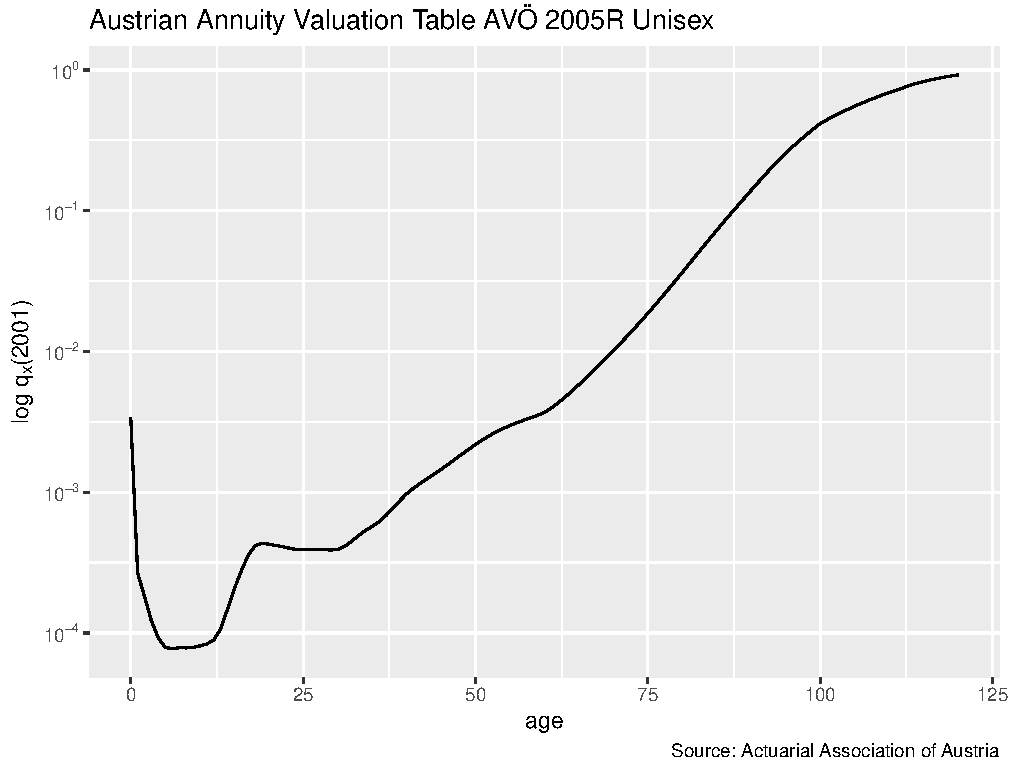
\includegraphics[width=0.9\textwidth]{figures/chapter_sensitivities/Austrian_Annuity_Valuation_Table/avoe_2005R_unisex}
	\caption{Logarithm of the yearly mortality defined by the Austrian Annuity Valuation Table AVÖ 2005R Unisex.}
	\label{fig:sensitivity_annuity_table_graph}
\end{figure}
Figure (\ref{fig:sensitivity_annuity_table_graph}) shows, for example, the graph of logarithmic mortality rates based on the values of the unisex mortality table from the Actuarial Association of Austria \cite{kainhofer2006new}. A high level of non-linearity can be observed, which naturally leads to greater challenges in the grouping process.

As known from life tables it is a bit more likely to die just after birth than a bit afterwards and the same is true for people aged around 20.  The exact ages where the probability of survival increases and the probability of death decreases when a person gets a year older depends heavily on the life table and the sex of the insured person. Whether the values for (\ref{equ:whole_life}) - (\ref{equ:temp_annuity}) will rise or fall when the age $x$ is increased by 1 year will therefore depend on $n$, $x$ and the sex of the insured person. To get a better insight into the portfolio, simulation runs for various parameters should be done. 
In figure (\ref{fig:sensitivity_age_claims}) the development of the yearly total claims is plotted against the duration of 25 years. The claims are the amount of money that must be paid to the policyholder at the time of an insured event multiplied by the probability that such an event will occur. Such events can be of all kinds, but the most common are, for example, the death of the insured person or a surrender of the contract. 

For a clearer chart the last cash flow which is the sum insured and therefore substantially larger than the yearly claims is omitted. We see that for younger people (green and red lines) the claims are almost identical in the first years and only deviate slightly at the end of the duration due to minor differences in the probabilities of death. For an insured person aged 60 we observe over the entire projection horizon considerably higher claims compared to younger policyholders. This gap between young and old policyholders which is mostly driven by mortality effects even increases with time. An insured person aged 60 which gets one year older faces in absolute values an higher increase in the mortality rate compared to an insured person aged 40 and so the claims will be higher in absolute values for the older person. This effect is partially compensated by lower surrender claims due to the higher mortality rates. If one compares the development of the claims also with respect to different interest rates, one can see in figure (\ref{fig:sensitivity_age_claims}) that there are hardly any differences between the values of 2\%, 3\% and 4\% shown. 

In figure (\ref{fig:sensitivity_age_premium}) the development of the booked premium at time 0 is plotted against the age. For policyholders aged between 15 and 30 the premium stays almost constant and then starts to increase exponentially. The increase of the premium is of exponential order due to the fact that the mortality rate is also increasing exponentially. Another fact that is not surprising is that the premium is the lower the higher the technical interest rate is, because the technical interest rate is used as a discount factor in (\ref{equ:whole_life}) - (\ref{equ:temp_annuity}). In figure  (\ref{fig:sensitivity_age_pvfp}) the present value of future profits (PVFP) at time 0 is plotted against the age. The PVFP is the higher the higher the entry age of the policyholder is, which is a counter intuitive relation at first sight. An analysis of the yearly cash flows for two different policyholders aged 15 and 70 reveals that this phenomenon is based on two different aspects as given in detail in table \ref{tab:PVFP_sensitivity}. 
\begin{enumerate}
	\item When the guaranteed interest rate is roughly equal to the investment return or even higher then it is more 		advantageous for the insurance company when the policyholder is older and therefore dies earlier because the difference between the guaranteed interest rate and the investment return need not to be financed over a long period. This leads to the observed fact that the PVFP is the lower the higher the technical interest rate is.
	\item The differences of the first and second order assumptions of the mortality rates are in absolute values the bigger the higher the age is, because in almost all cases the second order assumptions of of the mortality rates are just a fixed fraction of the first order assumptions. This directly leads to a higher risk margin and therefore to a higher premium for elder persons in absolute values as shown in column \textit{prem\_diff} in table \ref{tab:PVFP_sensitivity}. The  higher premium overcompensates the higher death claims and therefore increases the surplus in absolute values and leads to a higher present value of future profits. 
\end{enumerate}
In figure (\ref{fig:sensitivity_age_reserve}) the value of the reserve is plotted against the time. In all three cases the reserve is zero at the beginning and then starts to increase. This is due to the fact, that the valuation date of the projection is Q1 but the begin month of the policy is later. We see that for the ages of 15 and 30 the difference in the reserve is negligible for all different values of the technical interest rate. The reserve for a 45 year old person is almost identical to the one of younger policyholders at the first 10 years of the endowment but then increases at a slightly slower rate. For a person aged 60 we get a different picture because the reserve is not always monotonically increasing as it is true for the younger policyholders. The reserve increases after approximately 10 years at a much slower rate compared to the other policyholders and even starts to decrease after roughly 20 years. This effect can again be explained by the much higher morality rates in absolute values for older policyholders as time increases. Due to that fact the reserve is at the end of the projection horizon when the maturity claims are paid out for an older policyholder approximately half of the size as for a younger policyholder.

\begin{figure}
	\centering
	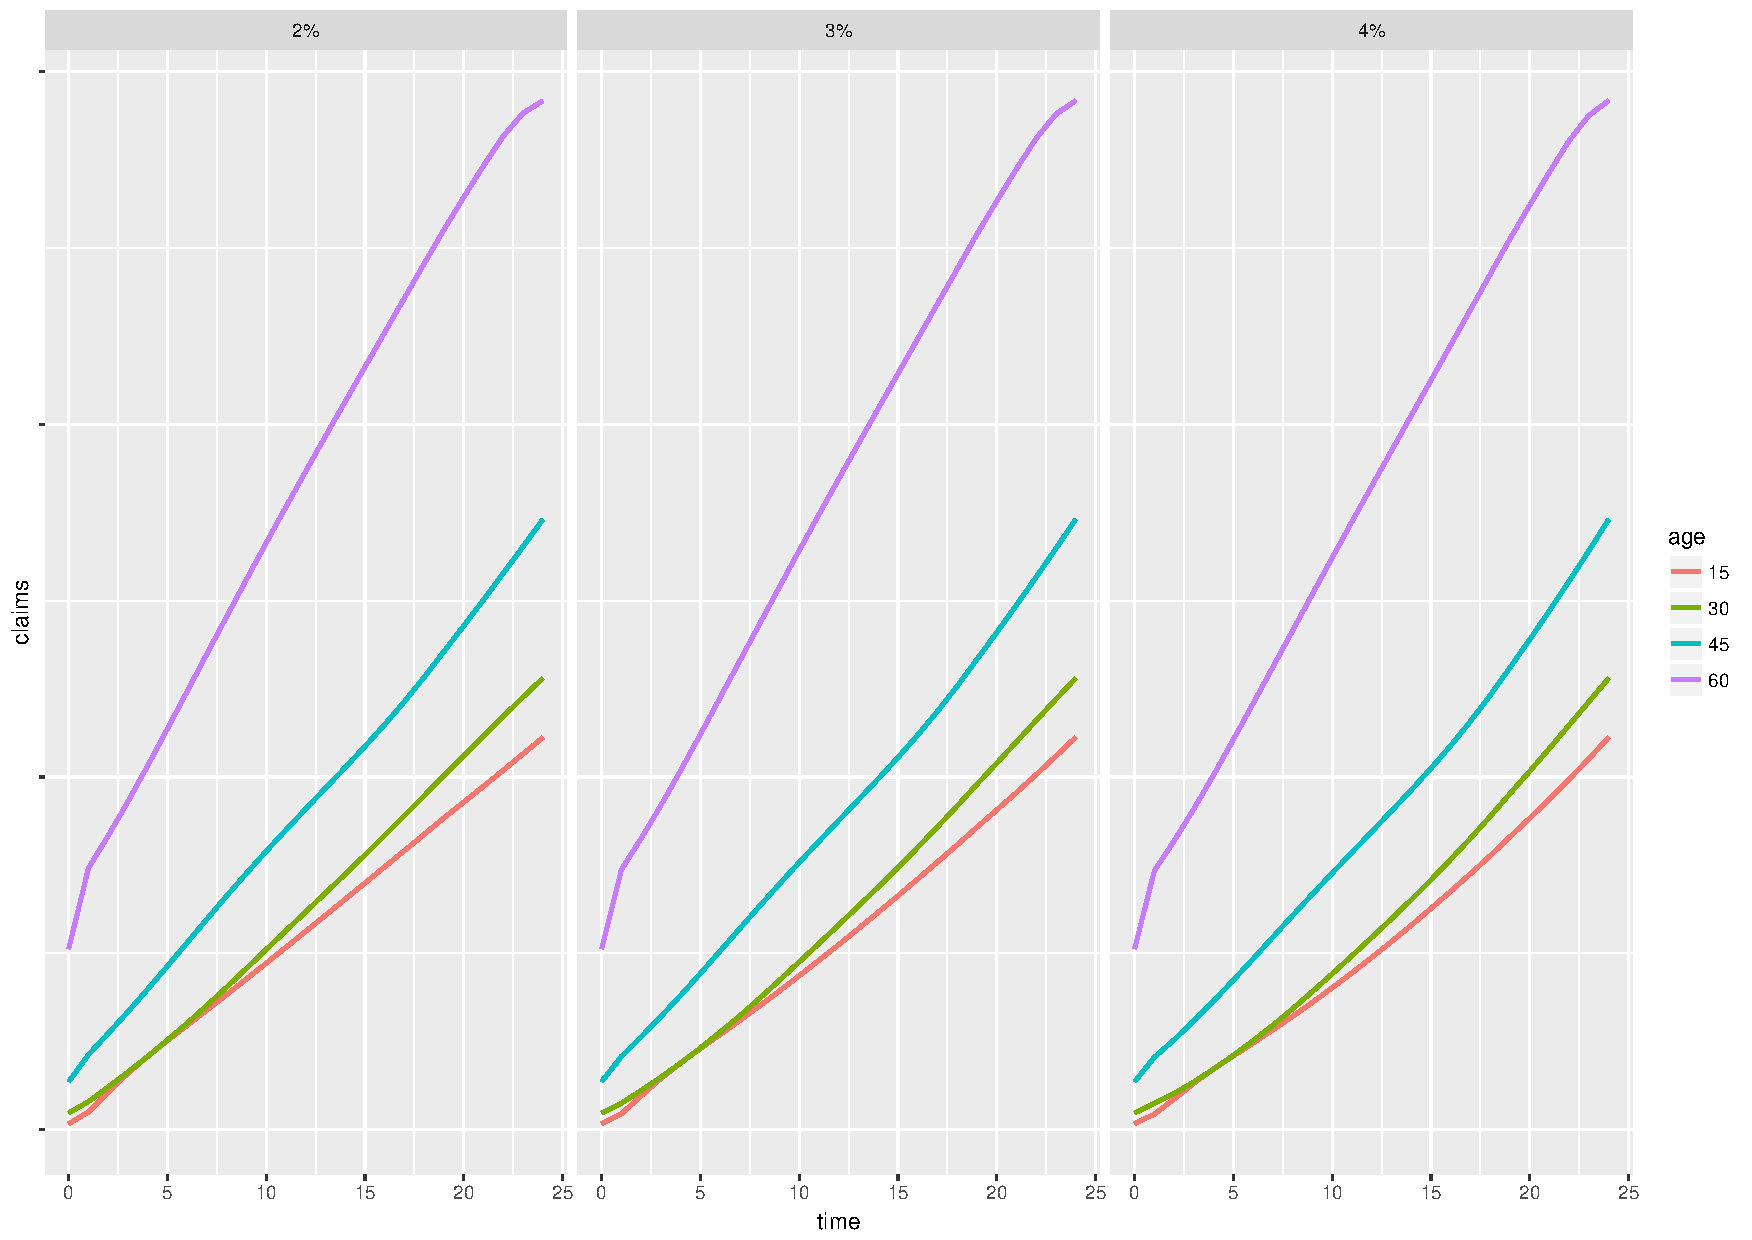
\includegraphics[width=0.9\textwidth]{figures/chapter_sensitivities/sensitivity_age_claims}
	\caption{Yearly cash flow for claims depending on the age and the technical interest rate.}
	\label{fig:sensitivity_age_claims}
	
	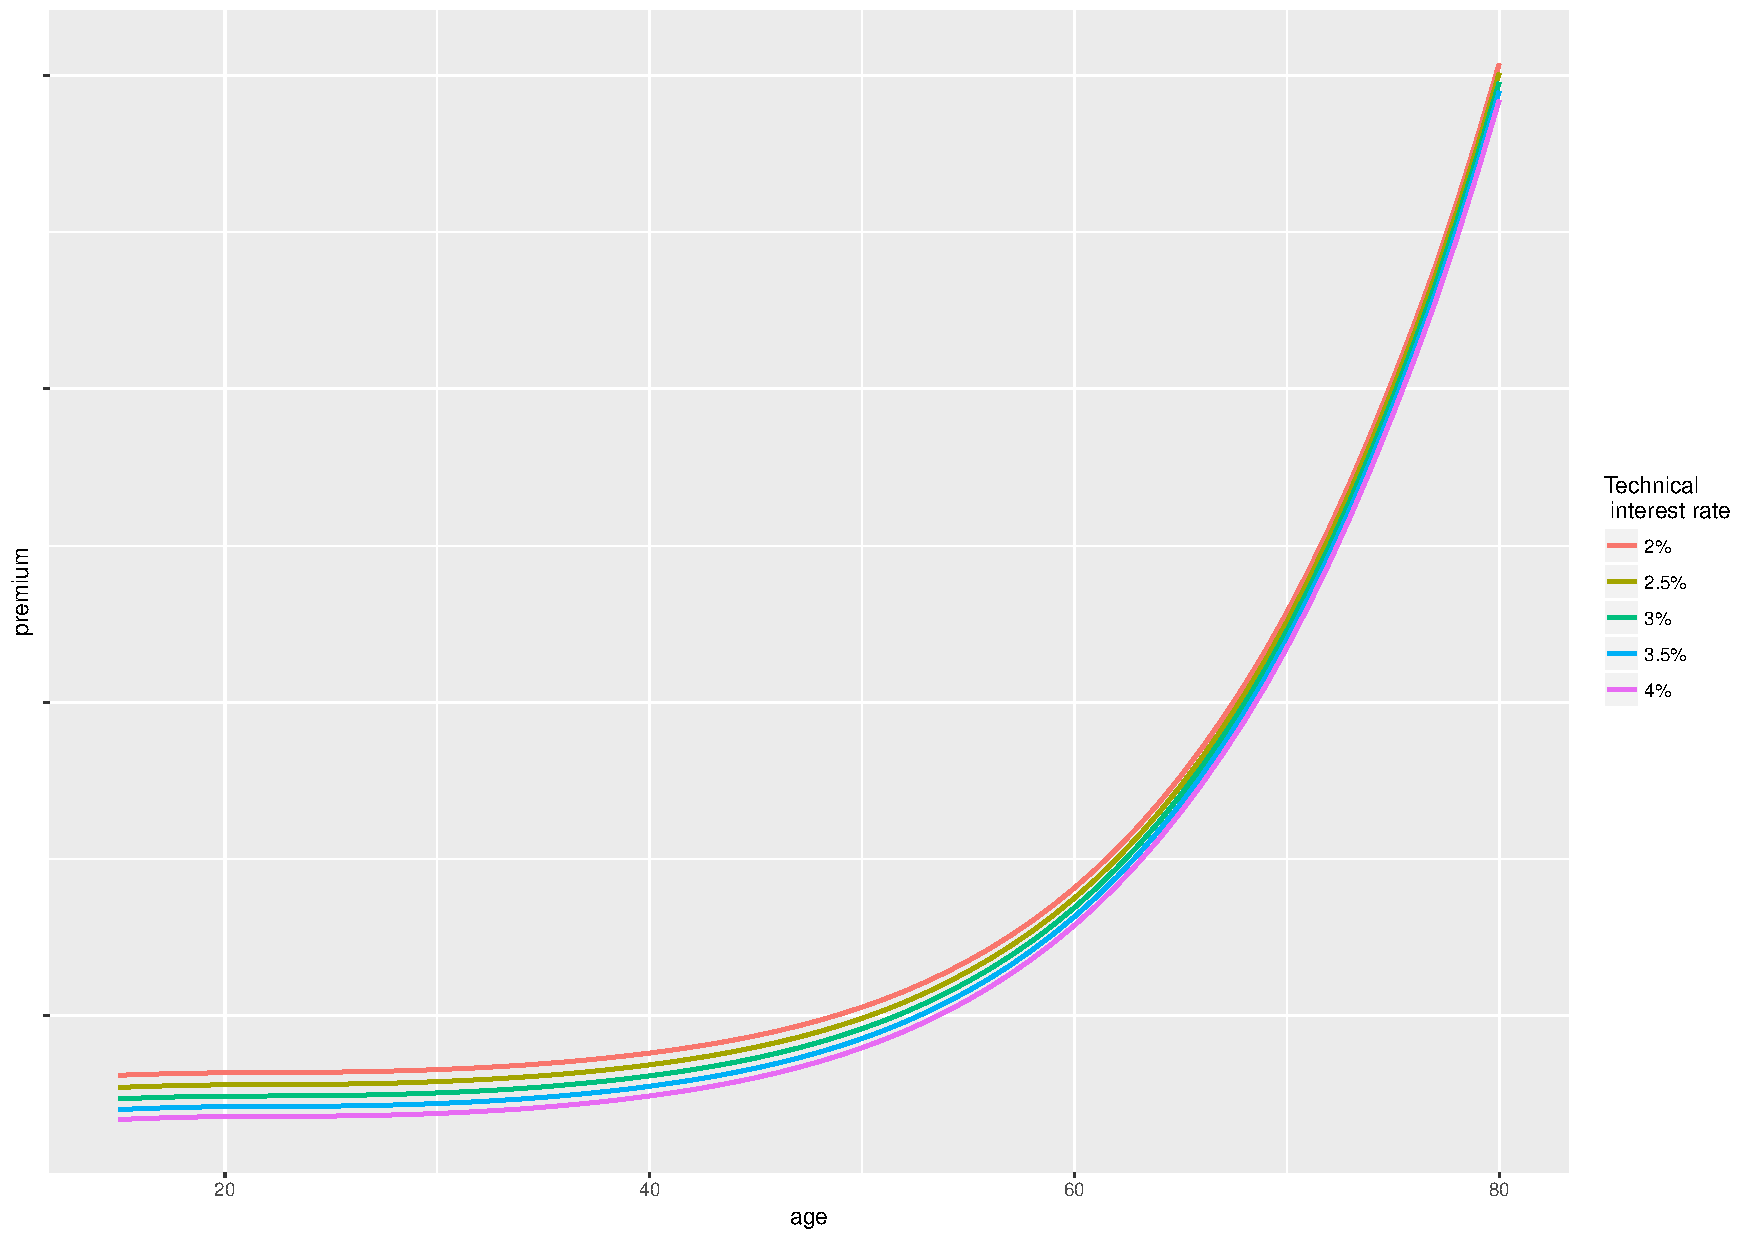
\includegraphics[width=0.9\textwidth]{figures/chapter_sensitivities/sensitivity_age_premium}
	\caption{Premiums depending on the age and the technical interest rate.}
	\label{fig:sensitivity_age_premium}
\end{figure}


\begin{figure}
	\centering
	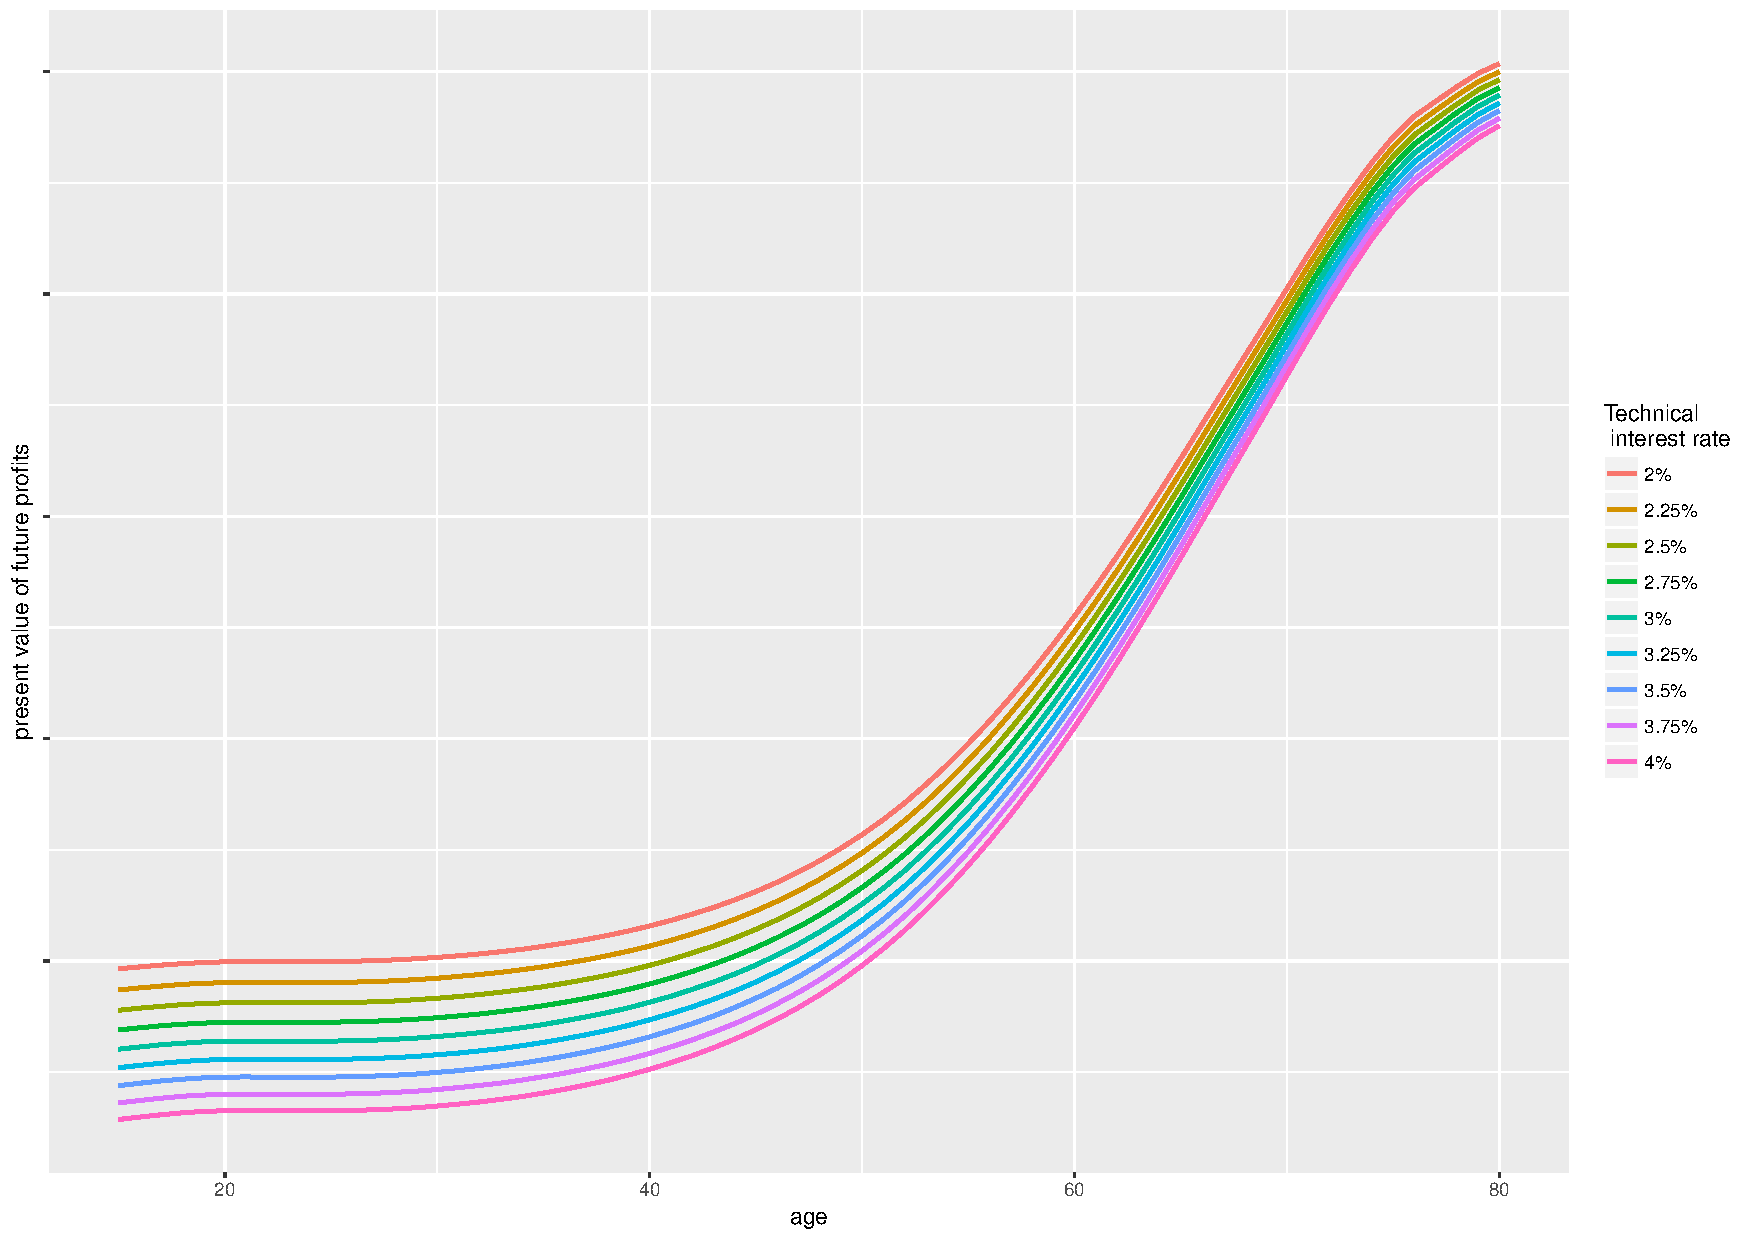
\includegraphics[width=0.9\textwidth]{figures/chapter_sensitivities/sensitivity_age_pvfp}
	\caption{Present value of future profits at time 0 depending on the age and the technical interest rate.}
	\label{fig:sensitivity_age_pvfp}

	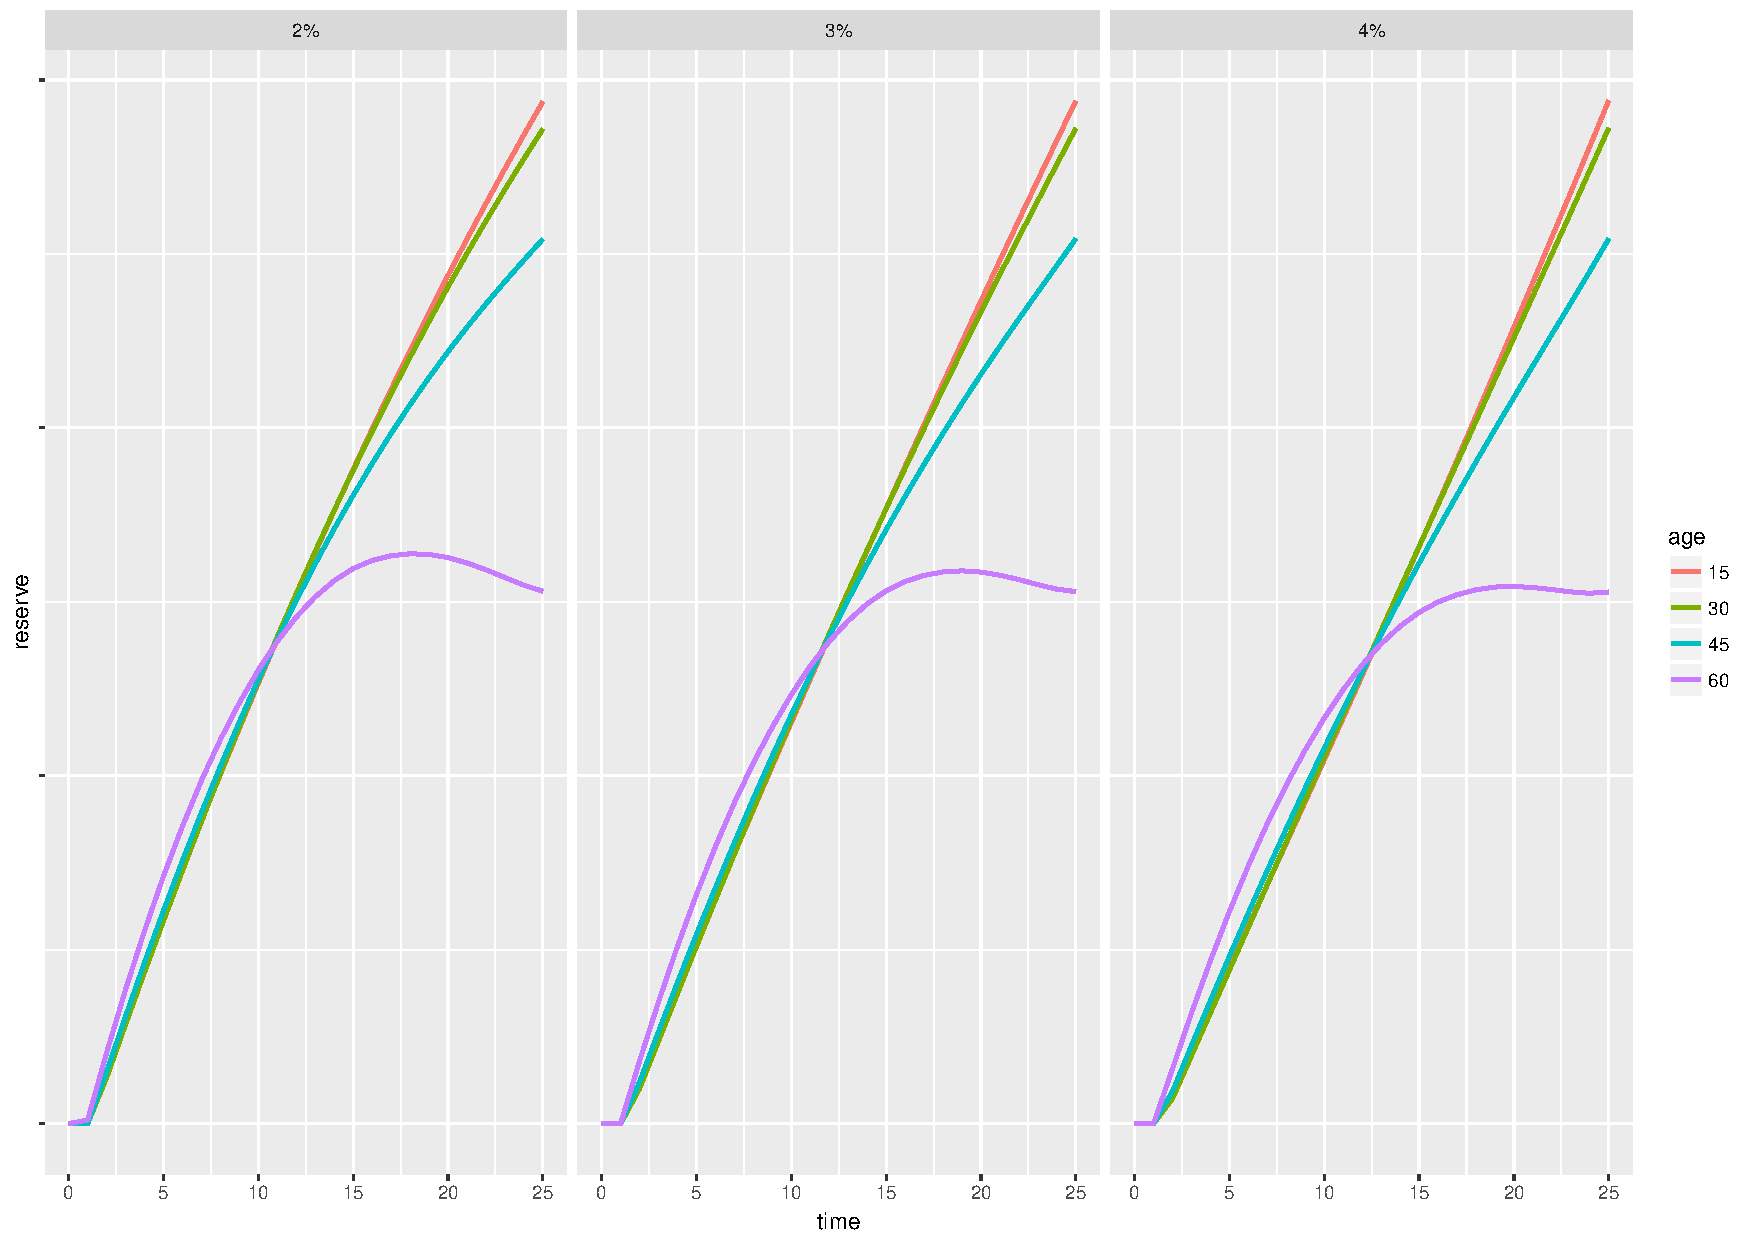
\includegraphics[width=0.9\textwidth]{figures/chapter_sensitivities/sensitivity_age_reserve}
	\caption{Yearly reserve depending on the age and the technical interest rate.}
	\label{fig:sensitivity_age_reserve}
\end{figure}


\section{Technical interest rate}
\label{sec:technical_interest_rate} 
The technical interest rate is one of the key assumptions in the life insurance business. It determines the factor by which the reserve and the savings premium increases during the contract period. After the contract has been concluded the technical interest rate is fixed and can't be changed by the insurance company. The maximum technical interest rate has been reduced dramatically by the Financial Market Authority in recent years from 4\% to 0.5\% as shown in table \ref{tab:interest_rates}.  The regulation of this upper bound is also relevant as it is often related to the minimum interest rate guaranteed to the policy holder. It is obvious that the higher the  technical interest rate, the higher the guaranteed benefit or the lower the premium will be. When the grouping algorithm forces policies from different product generations with same payout characteristics but different technical interest rates to be grouped together one important thing to be aware of are sensitivities. Another important aspect which need to be taken care of when policies with different technical interest rates are grouped together is the one of consistent management rules.  Take for example policy 1 with a technical interest rate of 2\% and a bonus rate of 2\% and policy 2 with a technical interest rate of 4\% and a bonus rate of 0\%. Lets assume that the two policies are similar and the grouped policy has a technical interest rate of 3\% and a bonus rate of 1\%. The total interest rate then is the same for the grouped and the ungrouped policies. Assume that the bonus rate is reduced by 1\% caused by a management decision. Then policy 1 has only a bonus rate of 1\% and policy 2 doesn't change at all, but the grouped policy has now a bonus rate of 0\%. The total interest rate is not the same for the grouped and the ungrouped policies which can potentially have major impacts on the projected cash flows. When the technical interest rate increases, the present value of future profits as well as the premium will decrease as shown in figure (\ref{fig:sensitivity_age_pvfp}) and (\ref{fig:sensitivity_age_premium}) respectively. This behaviour is not surprising at all, because as the technical interest rate rises the insurance company guarantees a higher benefit and this yields ceteris paribus to a lower PVFP. The reserve and the claims are not that much affected by an increase of the technical interest rate as shown in figure (\ref{fig:sensitivity_age_claims}) and (\ref{fig:sensitivity_age_reserve}) respectively.




\section{Duration}
\label{sec:duration}
The duration $n$ of an insurance contract is next to the age and the technical interest rate another main characteristic which need to be taken care of when a grouping process is carried out. In figure (\ref{fig:sensitivity_duration_claims}) the yearly claims except the last claim, which is the maturity claim, are shown for different ages. One obvious conclusion that can be derived is that the sum of all sorts of claims except the maturity claim is getting the higher the higher the age is. Another observation that can be made is that for any given time $t$ the claims are the higher the shorter the duration gets when we keep the age fixed. This is not surprising at all, because a shorter duration goes along with a higher premium (see figure (\ref{fig:sensitivity_duration_premium})) and a higher reserve (see figure (\ref{fig:sensitivity_duration_reserve})) which yields to higher claims for every fixed t.  In figure (\ref{fig:sensitivity_duration_premium}) we see that the premium is decreasing with an exponential order when the duration is increased. The difference between the premiums for policyholders with different ages is indistinguishable small for short term contracts and is getting bigger as duration increases. In figure (\ref{fig:sensitivity_duration_pvfp}) the present  value of future profits at time 0 is plotted against the duration of the contract. We see the same effect as in figure (\ref{fig:sensitivity_age_pvfp}) where contracts with higher ages lead to a higher PVFP. The effect of the absolute difference between the first and second order mortality assumptions is getting the bigger the longer the duration is and therefore the PVFP is getting the higher the longer the duration is. In the last sensitivity chart (\ref{fig:sensitivity_duration_reserve}) the reserve is plotted against the time for different values of $x$ and $n$. We see that for every time $t$ the reserve is the higher the shorter the duration is, because a shorter duration leads, ceteris paribus, to a higher premium which then results in a higher reserve. For short term contracts up to 10 years the reserve is approximately the same across different ages and is then getting the lower the higher the age and the  longer the duration is. After the sensitivity analysis has already provided the first important insights from the data, the next chapter discusses the first potential algorithm that can be used for the grouping of policies. 
\begin{figure}
	\centering
	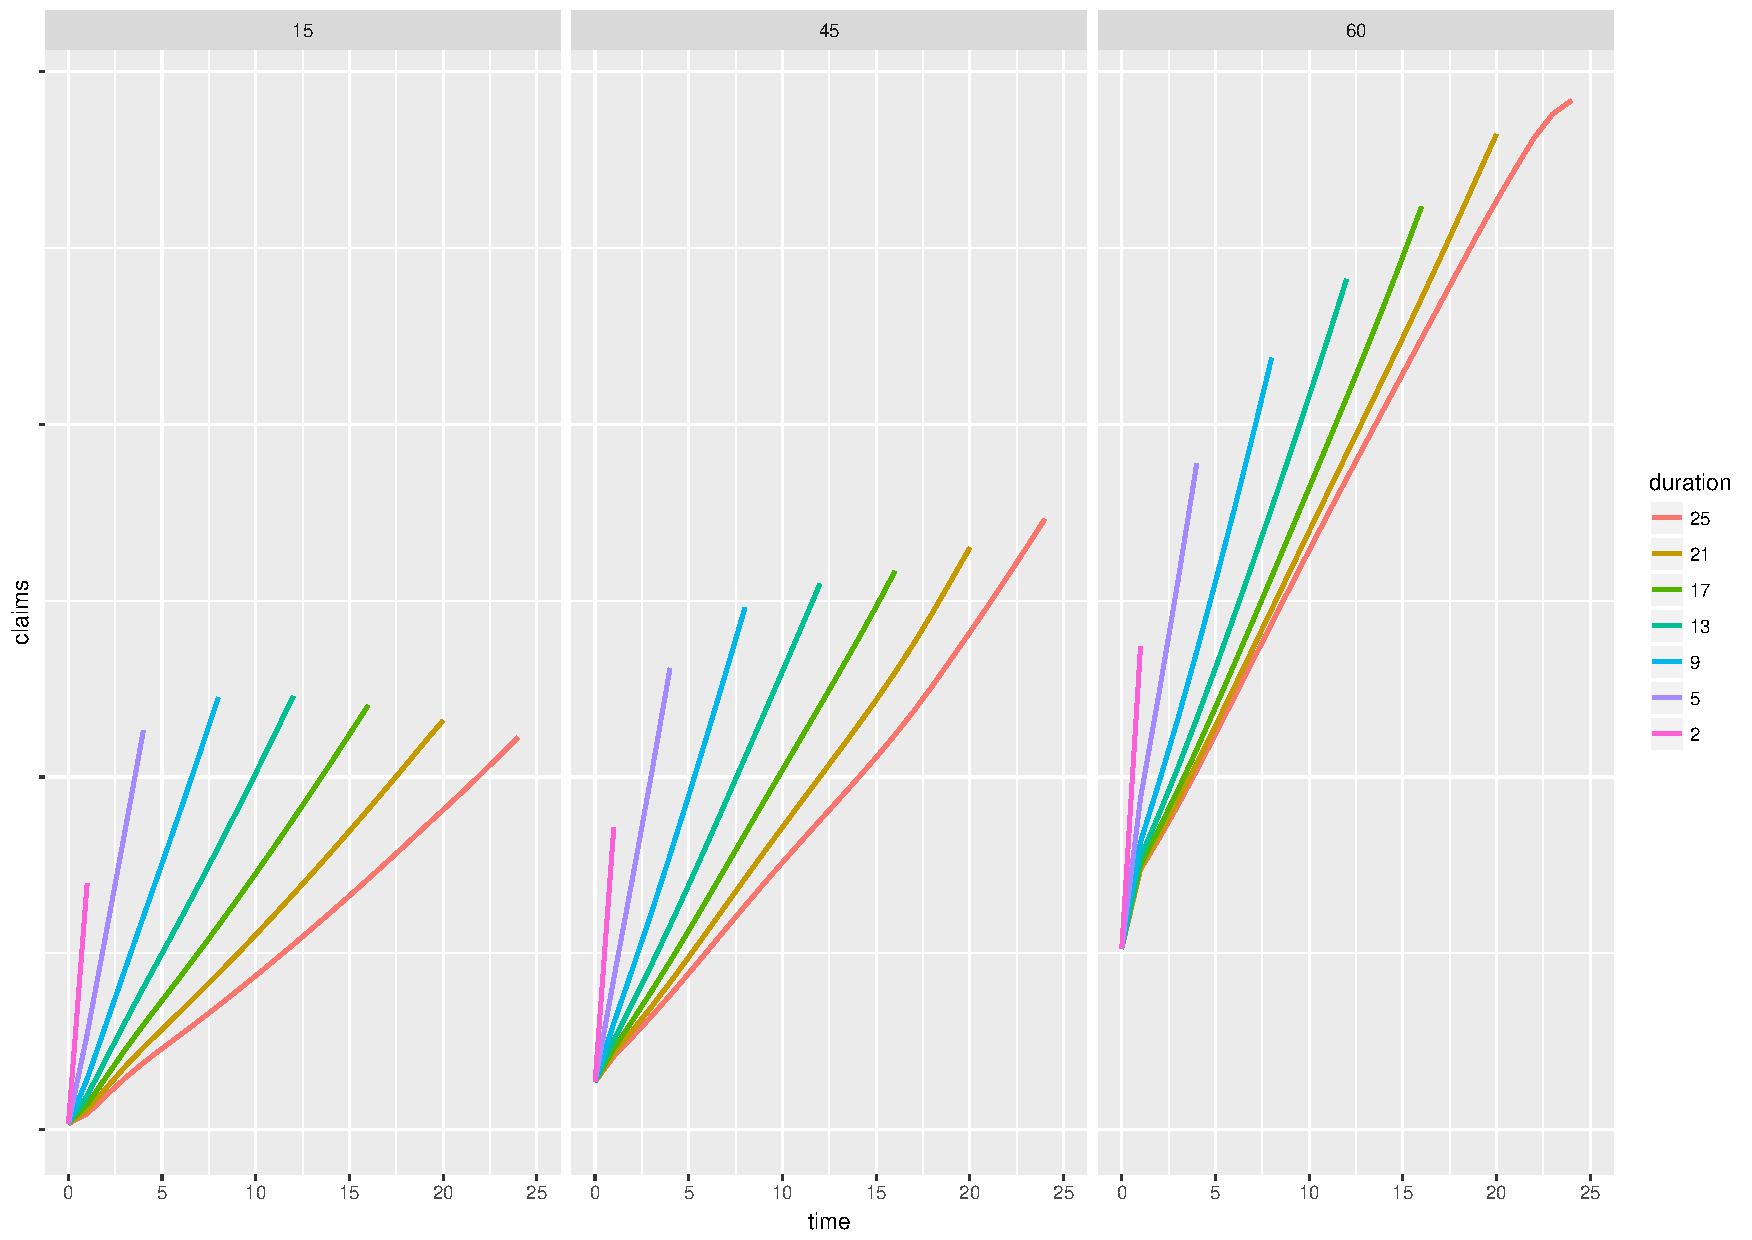
\includegraphics[width=0.9\textwidth]{figures/chapter_sensitivities/sensitivity_duration_claims}
	\caption{Yearly cash flow for claims depending on the duration and the age.}
	\label{fig:sensitivity_duration_claims}
%\end{figure}
%\begin{figure}
	\centering	
	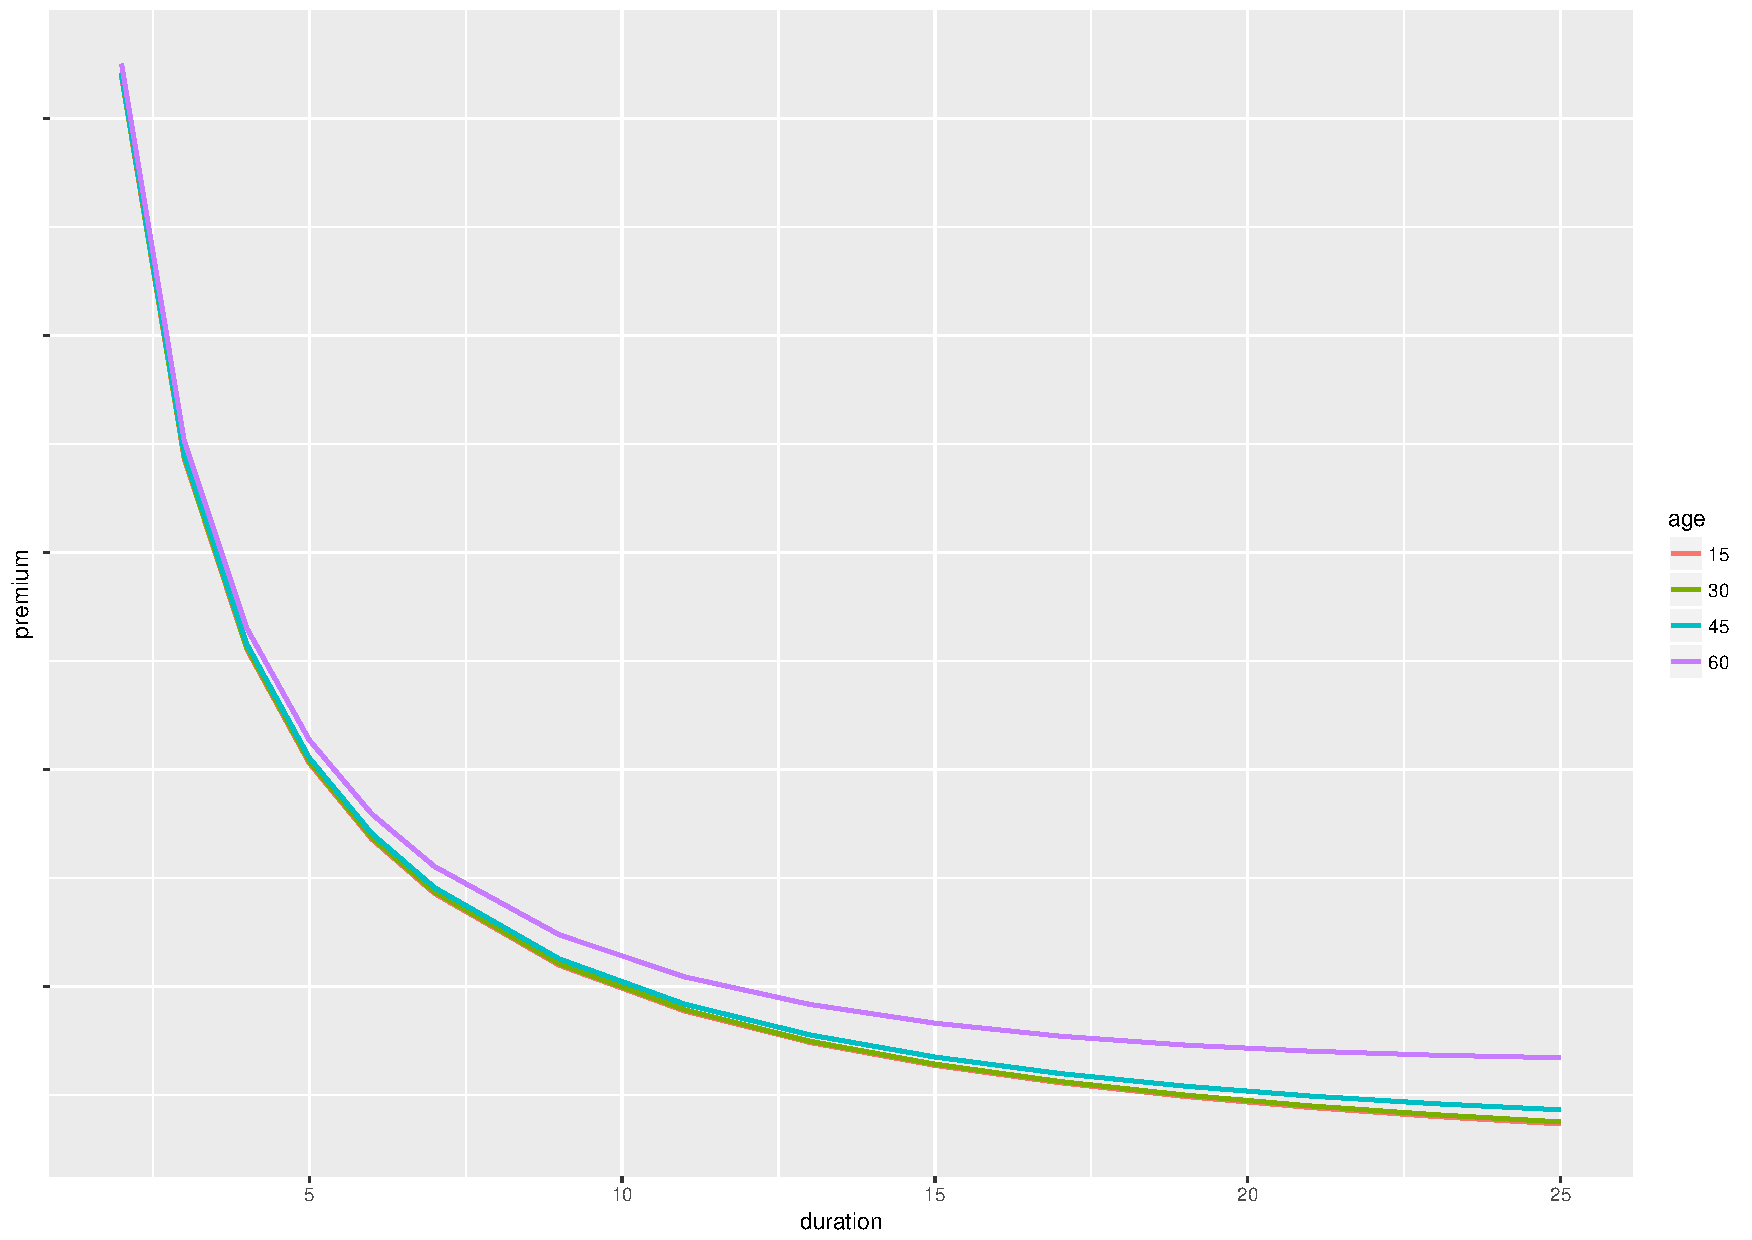
\includegraphics[width=0.9\textwidth]{figures/chapter_sensitivities/sensitivity_duration_premium}
	\caption{Premiums depending on the duration and the age}
	\label{fig:sensitivity_duration_premium}
\end{figure}



\begin{figure}
	\centering
	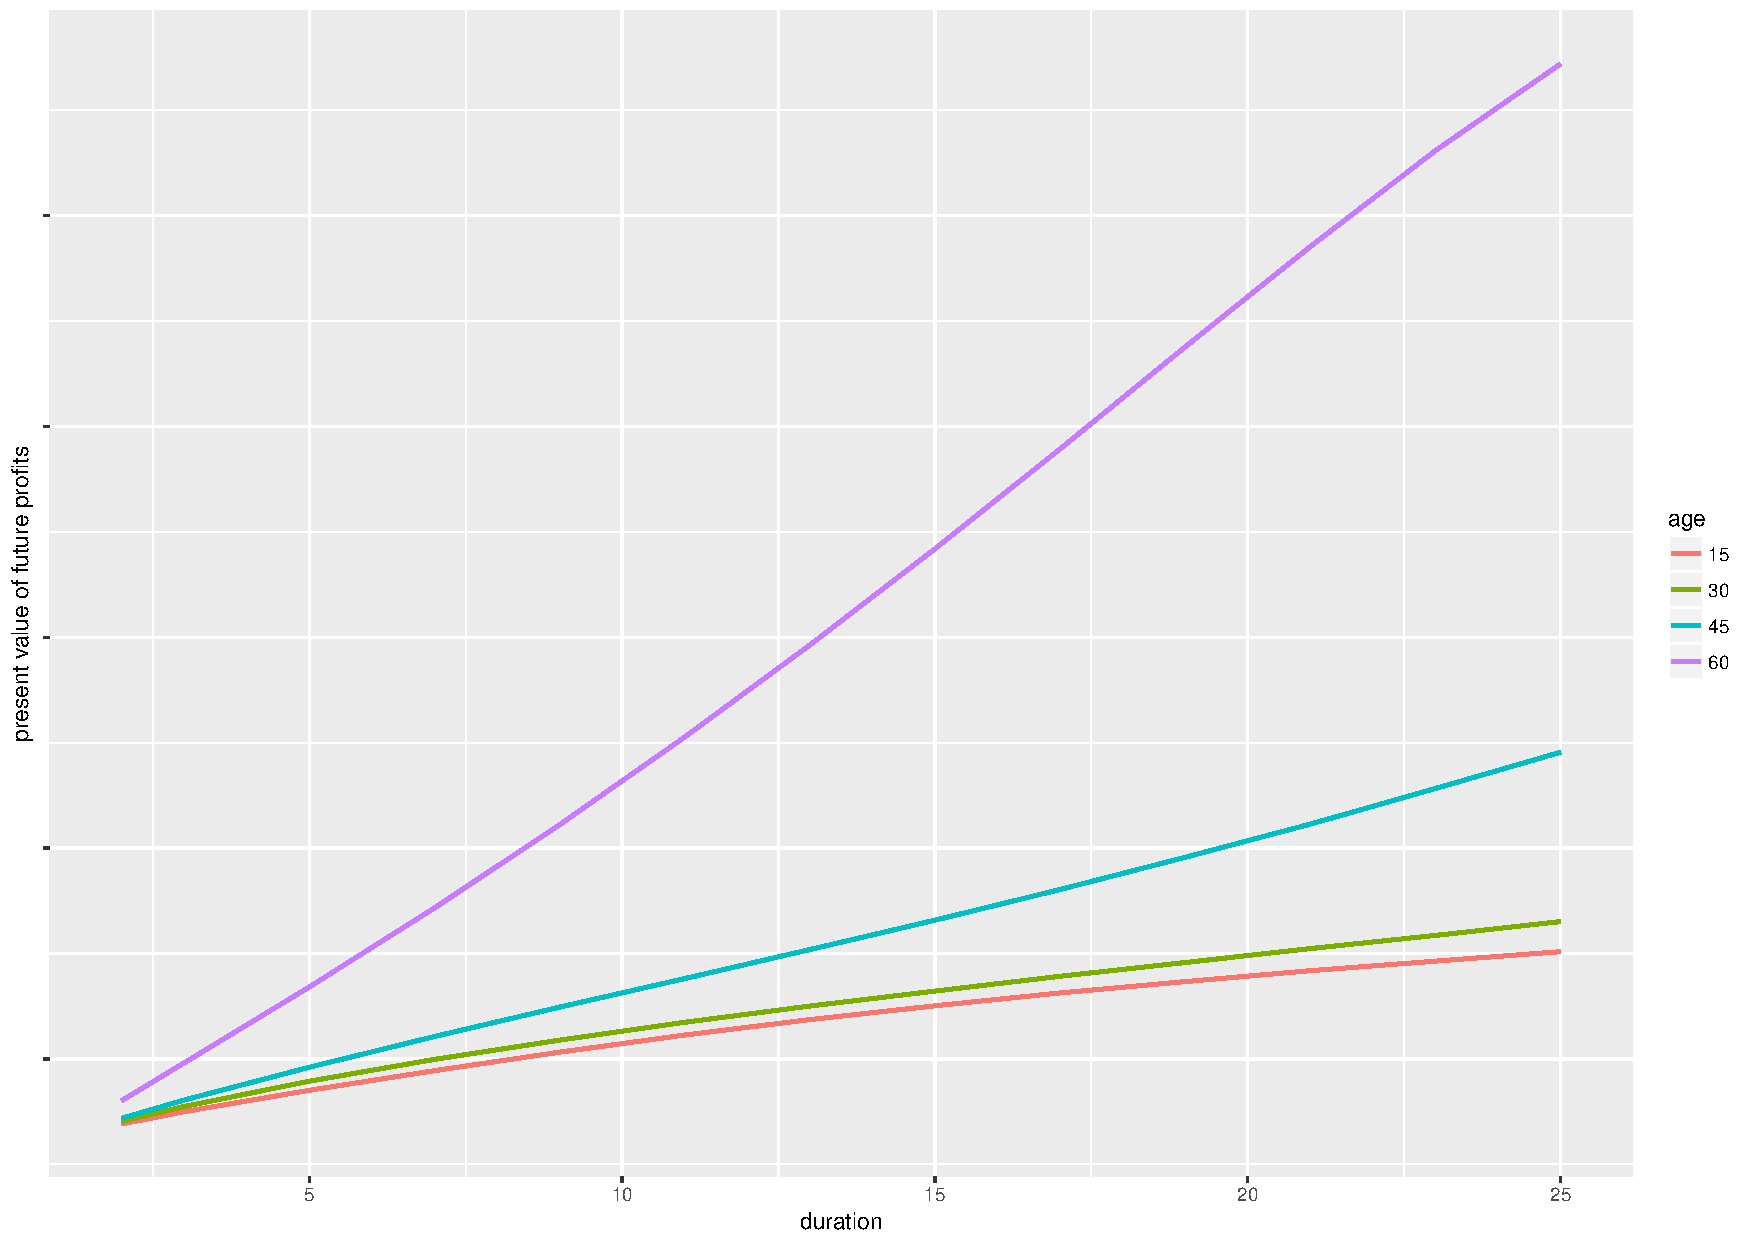
\includegraphics[width=0.9\textwidth]{figures/chapter_sensitivities/sensitivity_duration_pvfp}
	\caption{Present value of future profits at time 0 depending on the duration and the age.}
	\label{fig:sensitivity_duration_pvfp}

	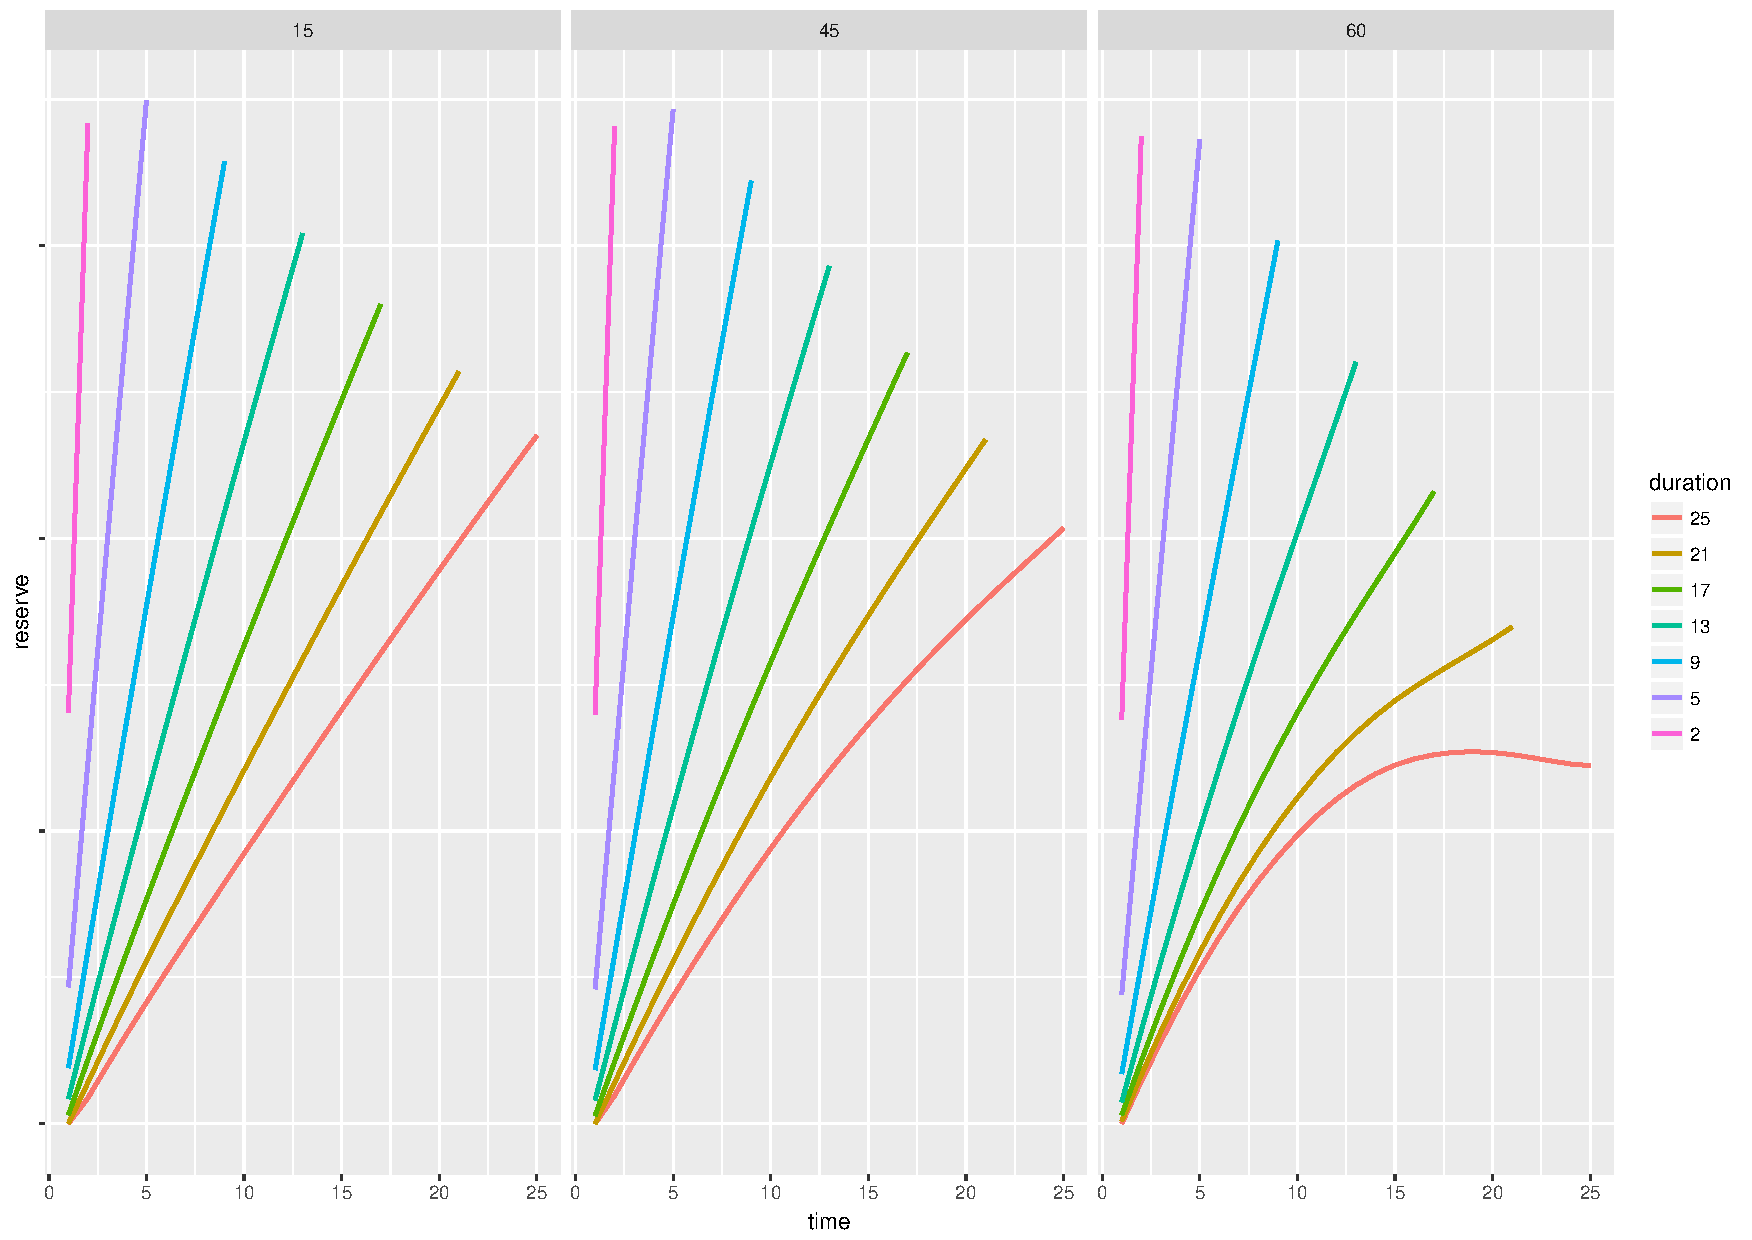
\includegraphics[width=0.9\textwidth]{figures/chapter_sensitivities/sensitivity_duration_reserve}
	\caption{Yearly reserve depending on the duration and the age.}
	\label{fig:sensitivity_duration_reserve}
\end{figure}
